\section{Results}
\label{sec:res}

\subsection{Misallocation in both directions}
\label{sec:both}

The five models, run under a registered design (Appendix~\ref{app:amendments}), misallocate their measurements in both directions.

The scripted rules set the yardstick (Table~\ref{tab:landscapes}). On the grid the guessing and model-guided rules
re-test \nGuessShare\% to \nBandHi\% of their slots, the \emph{scripted band}. The best final pick comes from the
informed rule, which is told which candidates are viable: a candidate worth \nInformedPick. On the two proteins, at the noise of the real assay (\emph{assay noise}), the
best scripted rule hardly re-tests at all: \nGbBestShare\% of slots on GB1 and none on PhoQ. With more noise,
re-testing pays there too (Section~\ref{sec:bench}).

Three models, Opus 4.7, Gemini 2.5 Flash and DeepSeek V3.1, over-confirm. On the grid they spend
\nShareOpusint\% to \nShareFlashint\% of their slots re-testing, far above the scripted band (Figure~\ref{fig:headline}),
and with every reading exact they still re-test half to nearly all of their slots, far more than exact readings
need (Appendix~\ref{app:grid}). Gemini 3.1 Pro under-confirms. It re-tests only \nShareProint\% of its slots, below the
band, so on the grid its pick is usually a candidate it measured only once. GPT-6.1 Sol sits just above the band.
On GB1 and PhoQ, where the best scripted rule re-tests at most 1\% of its slots, some models re-test less than on the grid, and every model still re-tests more than that rule, Gemini 3.1 Pro included (Table~\ref{tab:landscapes}). On the grid every model's final pick falls below the guessing rule's 7.87, and re-testing less did
not help Gemini 3.1 Pro or Sol pick better (Figure~\ref{fig:headline}). On GB1 Sol's lead over the guessing rule is uncertain,
and on PhoQ, a hard landscape for every strategy, three models are about level with it, and DeepSeek V3.1 and
Gemini 3.1 Pro pick worse (Appendices~\ref{app:atwo} and \ref{app:phoq}).


% Generated by scripts/make_table_landscapes.py from results/findings.json (results/landscapes_0an8.json and
% results/scripted_rules_best.json). Do not edit by hand; scripts/verify_paper_numbers.py regenerates it and
% fails on any difference.
\begin{table}[tbp]
\centering
\small
\caption{Re-testing share and true value of the final pick on each landscape, averaged over each model's campaigns. The three scripted rules are shown at their best setting.}
\label{tab:landscapes}
\begin{tabular}{lrrrrrr}
\toprule
 & \multicolumn{2}{c}{grid} & \multicolumn{2}{c}{GB1} & \multicolumn{2}{c}{PhoQ} \\
\cmidrule(lr){2-3}\cmidrule(lr){4-5}\cmidrule(lr){6-7}
 & share (\%) & pick & share (\%) & pick & share (\%) & pick \\
\midrule
Opus 4.7 & 74.9 & 7.62 & 63.3 & 4.78 & 62.8 & 1.89 \\
Gemini 2.5 Flash & 94.0 & 7.70 & 91.9 & 1.12 & 63.7 & 2.13 \\
DeepSeek V3.1 & 91.0 & 7.76 & 96.0 & 0.84 & 89.9 & 0.83 \\
GPT-6.1 Sol & 44.1 & 7.67 & 19.4 & 6.36 & 23.9 & 2.37 \\
Gemini 3.1 Pro & 14.0 & 7.69 & 11.1 & 4.90 & 14.7 & 1.72 \\
\midrule
guessing rule & 23.8 & 7.87 & 0.9 & \textbf{6.09} & 1.0 & 2.05 \\
informed rule & 23.3 & \textbf{8.00} & 0.0 & 6.02 & 0.0 & \textbf{2.63} \\
model-guided rule & 37.6 & 7.93 & 22.6 & 5.61 & 25.3 & 1.89 \\
\bottomrule
\end{tabular}
\end{table}


The over-confirmers lose through exploration (Figure~\ref{fig:loss}):
the best candidate they ever measured falls \nExplDeep{} to \nExplFlash{} short of the landscape's best, against 0.67
for the guessing rule, and among what they tested they pick almost perfectly. Gemini 3.1 Pro loses through selection. It explores about as well as the guessing rule and loses \nSelPro{} at
selection, against 0.23 for the guessing rule, because it often picks a candidate it measured only once. Sol loses about as much as the over-confirmers through exploration and less than the
guessing rule at selection.

\begin{figure}[tbp]
\centering
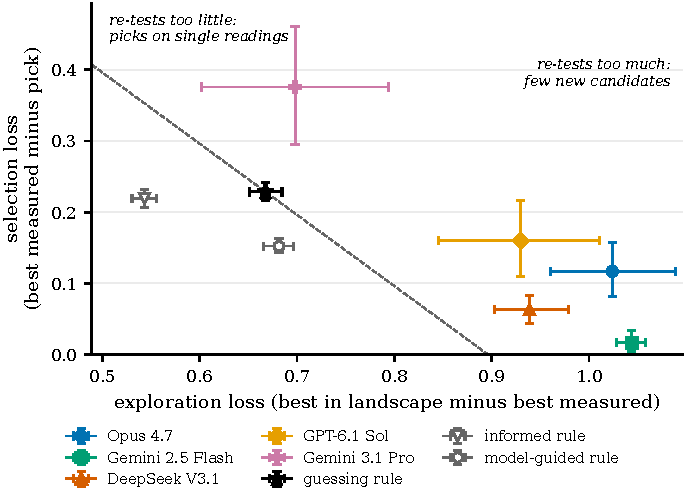
\includegraphics[width=0.68\textwidth]{fig_loss_directions.pdf}
\caption{Where each model's loss comes from, with 95\% intervals. Exploration loss: how far the best candidate
measured falls short of the landscape's best. Selection loss: how far the pick falls short of the best candidate
measured. The dashed line joins points with the guessing rule's total loss. The informed and model-guided rules are shown for reference; the informed rule is told which candidates are viable. Opus 4.7, Gemini 2.5 Flash and DeepSeek V3.1 measure too few candidates and pick well among them; Gemini 3.1 Pro measures as widely as the guessing rule and picks poorly.}
\label{fig:loss}
\end{figure}




\subsection{Over-confirmation}
\label{sec:why}

To understand why the three over-confirming models re-test so much (Figure~\ref{fig:headline}), we tested three
explanations on the grid. Each comes with an aid, given to these three models on the same seeds as their control, and
if an explanation holds, its aid should lower re-testing. GPT-6.1 Sol and Gemini 3.1 Pro do not over-confirm, so these
aids do not apply to them.
\begin{enumerate}
\item \textbf{Ledger.} \emph{They lose track of what they have measured.} The agent sees its history as one line per order, so a
candidate's readings are scattered across rounds. The ledger lists each measured candidate with its number of readings,
their mean and its standard error.
\item \textbf{Landscape note.} \emph{They do not know where to look next.} The agent is told nothing about how the landscape is built. The landscape note states how a candidate's score is built from its letters, and that a viable candidate's
neighbours are far more often viable than candidates in general.
\item \textbf{Menu.} \emph{They run out of new candidates worth trying.} The agent must name every new candidate itself, and most of
the new names it tries are rejected as non-viable. The Menu lists ten candidates the agent has never ordered, each one
letter from one of its three best, ranked by a simple model fitted to its own readings.
\end{enumerate}
The ledger and the landscape note changed re-testing by at most five percentage points (Figure~\ref{fig:fixes}a).
Three of these six changes were rises: the ledger for Opus 4.7 and DeepSeek V3.1, and the landscape note for DeepSeek V3.1. The Menu cut re-testing sharply in all three models, raised the best candidate they measured and worsened
their selection (Appendix~\ref{app:split}). The
over-confirmers re-test because they run short of candidates worth testing.

\begin{figure}[!t]
\centering
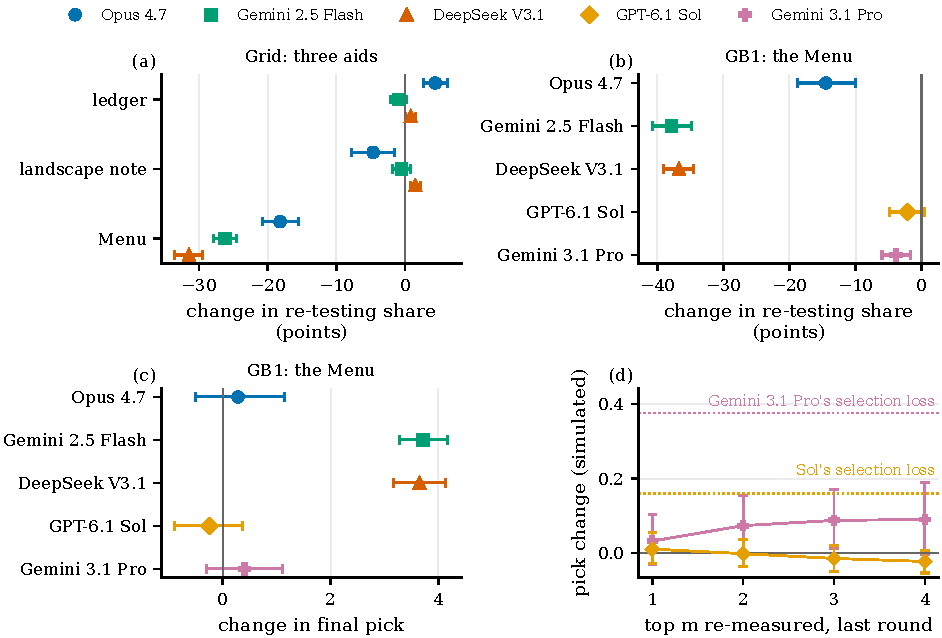
\includegraphics[width=\textwidth]{fig_fixes.pdf}
\caption{What we tested for each failure, each against the same model's control on the same seeds, with 95\% intervals.
\emph{Over-confirmation.} (a) The three aids on the grid, given to the three over-confirming models: change in re-testing
share. (b, c) The Menu on scrambled GB1, given to all five models: change in re-testing share and in final pick. It cuts
re-testing in the over-confirming models and lifts two of their picks by more than three units. It moves the re-testing of
Gemini 3.1 Pro and Sol by at most four points. \emph{Under-confirmation.} (d) The grid campaigns of Gemini 3.1 Pro and Sol, replayed with the last round spent re-testing the top $m$ candidates:
$m = 1$ re-tests the top one four times, and $m = 4$ re-tests each of the top four once. The y-axis is the change in the
true value of the final pick against the agent's own pick. Each dotted line is that model's selection loss, the most better checking could win back. Gemini 3.1 Pro
recovers about a quarter of it; Sol gains nothing.}
\label{fig:fixes}
\end{figure}


We then gave the Menu to all five models on scrambled GB1, built from real protein data, to test whether it carries
over and lifts the final pick. It cut re-testing again in the three over-confirmers (Figure~\ref{fig:fixes}b). Without it,
Gemini 2.5 Flash and DeepSeek V3.1 tested on average only \nGbDistinctFlash{} and \nGbDistinctDeep{} different candidates per
campaign. With it, their picks rose by more than three units of true value (Figure~\ref{fig:fixes}c). Almost all of the gain
came from finding better candidates, that is, from a smaller exploration loss.




For Gemini 3.1 Pro and Sol the Menu moved re-testing by at most four points and did not change their picks detectably
(Figure~\ref{fig:fixes}b and c), so they do not lack candidates. Gemini 3.1 Pro loses in how it picks, on single readings
(Section~\ref{sec:under}).

\subsection{Under-confirmation}
\label{sec:under}

Gemini 3.1 Pro under-confirms: it re-tests too little, so it often picks a candidate it measured only once and loses at selection (Figure~\ref{fig:loss}). If that is the cause, re-testing its top candidates before it picks should win back part
of the loss. Under-confirmation shows only on the grid, where re-testing pays, so we ran this test there. We asked one question:
had the agent spent its last round re-checking its best candidates, would its final pick have been better? To answer it
without calling the model again, we rebuilt each grid campaign of Gemini 3.1 Pro, and of Sol for comparison, from its log,
which reproduces every reading exactly. We then replaced the final round's four orders with re-tests of the top $m$
candidates by mean reading, under the same noise and failure rate. A fixed rule made the pick, the study's registered selection rule. It ranks
candidates by average reading, and pulls the average of a candidate with few readings toward the campaign's overall
average, so one lucky reading counts for less.

Gemini 3.1 Pro's pick improves as the re-tests are spread over more candidates, and at $m = 3$ it recovers about
\nAoneProRecoveredKthree\% of its selection loss (Figure~\ref{fig:fixes}d). This fits a true best that often sits just behind
a candidate with one lucky reading, so a second reading lets it overtake. The same rule applied to its unchanged readings gains almost nothing (Appendix~\ref{app:aone}), so the gain comes
from the extra readings. The gain stays small because Pro ends a campaign with
dozens of candidates measured only once, and four slots can re-check only a few. Sol gains nothing, since its top
candidates already have several readings each. Its curve dips slightly below zero because the replay gives up the new
candidates its real final round would have tried. In an exploratory run, re-testing over the last two rounds
recovered about as much as the last round alone.
